\section*{Introducció}

Aquest projecte té com a objectiu dissenyar i implementar una eina d'anàlisi estàtica de software mitjançant grafs de dependències i fluxos d'execució.

\section*{Contextualització}
\subsection*{Anàlisi estàtica de software}
L'anàlisi estàtica de software és una tècnica que consisteix a examinar el codi font d'un programa sense executar-lo. Aquesta tècnica té l'objectiu d'identificar errors, vulnerabilitats i altres problemes relacionats amb el codi \cite{static_code_analysis_jetbrains}. A més, permet analitzar les dependències entre els diferents components del programa i els fluxos d'execució, ajudant a identificar altres possibles problemes. Un altre avantatge d'aquesta anàlisi és que, en cas d'haver de modificar alguna part del codi, permet identificar quines altres parts poden veure's afectades.


\subsection*{Representació del codi i arbres sintàctics}
L'anàlisi estàtica de software no treballa habitualment directament sobre el codi font, sinó sobre una representació estructurada d'aquest. Una de les representacions més habituals és l'AST (Abstract Syntax Tree), un arbre que representa l'estructura sintàctica del programa i les relacions entre els seus diferents elements. Tanmateix, l'AST no conté tota la informació necessària per analitzar el comportament del programa, ja que el seu objectiu principal és representar-ne l'estructura sintàctica. Per exemple, l'ordre i les possibles rutes d'execució del programa requereixen altres representacions, com els grafs de flux d'execució.

Per obtenir l'AST, el codi font passa per diferents fases d'anàlisi. Inicialment, l'anàlisi lèxica divideix el codi en tokens, identificant i classificant les diferents unitats lèxiques que el formen. Aquest procés es podria comparar amb agafar una frase i identificar la categoria de cadascuna de les seves paraules. Posteriorment, l'anàlisi sintàctica utilitza aquests tokens per comprovar si compleixen les regles gramaticals del llenguatge i construir una representació de la seva estructura, com l'AST. Seguint amb l'analogia lingüística, aquesta fase seria equivalent a comprovar si les paraules d'una frase estan ordenades d'acord amb les regles gramaticals.

Un cop comprovada l'estructura sintàctica, es pot dur a terme l'anàlisi se\-màntica, que comprova que les construccions del programa tinguin un significat vàlid segons les regles del llenguatge. Per exemple, intentar modificar el valor d'una variable immutable pot ser sintàcticament correcte, però donar lloc a un error semàntic, ja que aquesta operació no és vàlida. De manera similar, en l'analogia lingüística, una frase pot tenir una estructura sintàctica vàlida, però contenir combinacions de paraules que no siguin correctes; com podria ser un article femení acompanyant un nom masculí.

A partir d'aquestes representacions i de la informació obtinguda durant les diferents fases d'anàlisi, les eines de processament de codi poden construir estructures que permetin realitzar diferents tipus d'anàlisi estàtica \cite{clang_llvm}\cite{balapriya_ast}.

\subsection*{Grafs de dependències i fluxos d'execució}
En l'àmbit de l'anàlisi estàtica de codi és molt valuós saber no només com s'estructura el codi, sinó també com es relacionen els diferents elements entre si. Per analitzar aquestes relacions, existeixen els grafs de dependències, a partir dels quals podem observar i analitzar quines afectacions pot tenir una certa modificació en la resta del codi, quines instruccions depenen de les dades produïdes per una instrucció prèvia o, fins i tot, identificar de quina manera es podria paral·lelitzar l'execució del programa \cite{gfg_dependencygraph}.

Una altra representació molt interessant són els grafs de flux d'execució. Aquests grafs tenen una missió molt simple: representar els possibles camins de control que pot seguir l'execució d'un programa. Aquesta informació és molt útil per diverses raons. En primer lloc, permet calcular la complexitat ciclomàtica del programa, que pot utilitzar-se com a indicador de la seva complexitat estructural.

En segon lloc, és útil de cara a testejar el software, ja que permet identificar els diferents camins i condicions de control que poden produir-se durant l'execució. D'aquesta manera, es poden dissenyar proves que cobreixin diferents camins d'execució, incloent-hi casos extrems.

Finalment, de cara a depurar o mantenir el codi, aquesta representació ajuda a acotar la quantitat de camins que s'han d'analitzar. Això pot evitar una pèrdua excessiva de temps a l'hora d'identificar quin camí d'execució està donant problemes o quines parts del codi poden veure's afectades per una modificació \cite{gfg_controlflowgraph}.

\subsection*{Detalls d'implementació}
El desenvolupament del projecte es durà a terme utilitzant C\#. Aquest llenguatge, en ser fortament tipat, de tipatge estàtic i orientat a objectes, proporciona una base sòlida per implementar de forma clara i estructurada les classes i abstraccions requerides pel disseny proposat. A més, la plataforma .NET proporciona eines per al testing i la configuració del projecte, així com suport multiplataforma i una bona integració amb entorns d'integració contínua com GitHub Actions. Finalment, les consultes mitjançant LINQ seran útils a l'hora de realitzar les diferents operacions necessàries per als tipus d'anàlisi proposats.

A més, C\# serà el primer llenguatge analitzat, ja que disposa de Roslyn, una plataforma de compilació desenvolupada per Microsoft que, a més de proporcionar informació sintàctica mitjançant l'AST, permet accedir a una gran quantitat d'informació semàntica sobre el codi. Aquesta informació serà especialment útil per implementar les primeres transformacions cap a la representació intermèdia i els diferents tipus d'anàlisi. Al mateix temps, disposar d'informació semàntica completa sobre el codi analitzat permetrà utilitzar Roslyn com a primera referència per validar la correcció dels resultats obtinguts per l'eina desenvolupada.


\subsection*{Eines i enfocaments existents}
L'anàlisi estàtica de codi és un camp que té un ampli desenvolupament al darrere i, per tant, ja existeixen diverses eines que duen a terme aquest tipus d'anàlisi. Cada una, però, té un funcionament i uns objectius una mica diferents. Per exemple, Tree-sitter permet obtenir arbres sintàctics de diferents llenguatges \cite{tree_sitter}, mentre que Joern utilitza Code Property Graphs com a representació intermèdia comuna per a l'anàlisi de codi \cite{joern_cpg}. CodeQL ofereix una plataforma més completa orientada a realitzar consultes i anàlisis sobre bases de codi \cite{codeql}. També existeixen propostes com Koncepto, que introdueixen una capa d'abstracció sobre el codi per representar conceptes i invariants d'alt nivell \cite{koncepto}.

Per tant, ja hi ha diverses eines en aquest àmbit que duen a terme, de forma més o menys completa, l'anàlisi de codi. Aleshores, la proposta d'aquest projecte no pretén substituir ni millorar directament cap d'aquestes eines, sinó estudiar i implementar una abstracció pròpia centrada a representar conceptes comuns de diferents llenguatges, com poden ser classes, funcions, templates i interfícies, tenint en compte les seves respectives diferències, o relacions d'herència. L'objectiu és desacoblar tant com sigui possible les característiques específiques de cada llenguatge de les representacions i anàlisis posteriors, mitjançant una capa intermèdia comuna encarregada de proporcionar les abstraccions corresponents. Així doncs, es podrà estudiar fins a quin punt és possible utilitzar una representació comuna per a diferents llenguatges sense perdre precisió ni capacitat d'anàlisi.

A més, diverses empreses del sector, com JetBrains, desenvolupen eines d'anàlisi i comprensió de codi, fet que evidencia l'interès existent en aquest tipus de tecnologies tant en l'àmbit acadèmic com en l'àmbit industrial \cite{jetbrains_inspectopedia}.


\subsection*{Context i motivació del projecte}
Tot i l'existència d'eines d'anàlisi estàtica, aquestes poden estar orientades a objectius concrets o limitar-se a determinats llenguatges i tipus d'anàlisi. En aquest context, aquest projecte proposa el desenvolupament d'una eina centrada en la representació de les relacions entre els diferents elements del codi mitjançant una abstracció comuna als diferents llenguatges analitzats, permetent posteriorment realitzar diferents tipus d'anàlisi sobre aquesta representació.

A més, es proposa una solució visual i senzilla, amb l'objectiu de facilitar-ne l'ús i permetre una interacció més còmoda per part de l'usuari.

Per últim, aquesta abstracció permet unificar la representació dels diferents elements del codi, deixant oberta la possibilitat d'incorporar l'ús de tècniques d'intel·ligència artificial en un futur.


\section*{Objectius}

\begin{objectius}

% =========================================================
% A. ARQUITECTURA I ABSTRACCIÓ
% =========================================================

\objectiu{
 Dissenyar una arquitectura modular i extensible per a una eina d'anàlisi estàtica de software.
}{
 Aquesta arquitectura permetrà desacoblar el processament específic de cada llenguatge dels mecanismes de construcció de grafs i anàlisi estàtica, facilitant la incorporació de nous llenguatges i la reutilització dels components comuns.
}

\objectiu{
 Desenvolupar una representació intermèdia capaç de modelar conceptes comuns de diferents llenguatges de programació.
}{
 Es definirà una representació intermèdia que permeti abstraure les característiques compartides entre diferents llenguatges, preservant la informació rellevant per a l'anàlisi estàtica. Es prioritzaran inicialment llenguatges amb característiques similars, com C\#, C++ o Java, i posteriorment es podrà estudiar la seva generalització a llenguatges amb característiques diferents, com Python.
}

\objectiu{
 Avaluar la capacitat de l'arquitectura per desacoblar els parsers dels components d'anàlisi i facilitar-ne la reutilització.
}{
 Es comprovarà que diferents parsers poden utilitzar una mateixa representació intermèdia i els mateixos components de construcció de grafs i anàlisi, sense necessitat de modificar-ne la implementació. També s'avaluarà l'esforç necessari per incorporar nous llenguatges, tenint en compte el codi afegit, els components reutilitzats i les modificacions requerides sobre l'arquitectura existent.
}


% =========================================================
% B. IMPLEMENTACIÓ I FUNCIONALITATS
% =========================================================

\objectiu{
 Implementar una primera versió de l'eina mitjançant un parser de C\#.
}{
 C\# ofereix un sistema de tipus estàtic i un model orientat a objectes que faciliten el desenvolupament d'una arquitectura modular i extensible. A més, l'ecosistema .NET proporciona eines madures per al desenvolupament i testing de l'eina.
}

\objectiu{
 Desenvolupar mecanismes de construcció de grafs de dependències i fluxos de control.
}{
 Aquests mecanismes permetran representar les relacions entre els diferents elements del programa, així com les possibles seqüències d'execució dins dels mètodes. Els grafs generats serviran com a base per implementar diferents funcionalitats d'anàlisi estàtica.
}

\objectiu{
 Implementar funcionalitats d'anàlisi estàtica sobre els grafs generats.
}{
 Es desenvoluparan funcionalitats que permetin analitzar les dependències entre els diferents components del programa, identificant el grau d'acoblament, possibles dependències circulars o innecessàries i l'impacte potencial de les modificacions. També s'analitzaran els fluxos de control per identificar possibles punts o camins crítics.
}

\objectiu{
 Representar visualment els resultats mitjançant grafs.
}{
 Aquesta representació permetrà als usuaris analitzar i comprendre de manera senzilla els resultats obtinguts per l'eina, així com identificar visualment possibles problemes o oportunitats de millora en el software.
}


% =========================================================
% C. VALIDACIÓ I AVALUACIÓ
% =========================================================

\objectiu{
 Garantir el correcte funcionament de l'eina amb un subconjunt representatiu dels elements dels llenguatges implementats.
}{
 Aquest objectiu permet delimitar l'abast del projecte i establir un conjunt concret de funcionalitats sobre les quals avaluar el correcte funcionament de l'eina. Per fer-ho, es definiran diferents casos de prova que cobreixin les construccions dels llenguatges implementades, incloent-hi variants i situacions que puguin presentar dificultats durant el processament.

 Els resultats obtinguts es compararan amb una referència, ja sigui mitjançant resultats verificats manualment o eines existents, utilitzant mètriques com la precisió, el recall i l'F1-score. També s'analitzarà la cobertura dels elements del llenguatge, diferenciant entre aquells que es processen correctament, parcialment o incorrectament.
}

\objectiu{
 Avaluar el rendiment i l'escalabilitat de l'eina en projectes de diferents dimensions i complexitats.
}{
 Aquest objectiu permetrà estudiar el comportament de l'eina en escenaris pràctics i identificar possibles limitacions. Per avaluar-lo, es definiran diferents casos de prova sobre projectes reals o representatius de diverses dimensions.

 Es mesurarà el rendiment dels diferents components del sistema, com ara el processament del codi font, la construcció de la representació intermèdia i la generació dels grafs. Es tindran en compte mètriques com el temps d'execució, el consum de memòria i la mida de les estructures generades, estudiant-ne l'evolució en funció de la dimensió dels projectes analitzats.
}

\objectiu{
 Analitzar la utilitat de l'eina en la detecció i comprensió de problemes estructurals del software.
}{
 Aquest objectiu permetrà avaluar la utilitat de l'eina en la detecció i comprensió de problemes estructurals del software, així com en la identificació de punts de millora. Per avaluar-ho, es compararan les tasques d'anàlisi realitzades amb l'eina i sense, observant els problemes detectats i el temps necessari per identificar-los.
}

\end{objectius}

\section*{Metodologia}
El desenvolupament del projecte seguirà una metodologia iterativa i incremental. Inicialment, es dissenyarà una arquitectura i les principals funcionalitats de l'eina, que posteriorment seran implementades. Durant aquest procés, s'anirà avaluant el correcte funcionament de les característiques implementades mitjançant proves, a més de les reunions de seguiment periòdiques amb el tutor. En cas de detectar errors o mancances, es revisarà el disseny per tal de corregir-los o incorporar els elements necessaris. L'objectiu principal d'aquesta metodologia és mantenir un desenvolupament àgil i flexible, prioritzant la netedat i la qualitat del software desenvolupat.
Quant als objectius, aquests serviran per marcar les fites del projecte, ja que cada un comporta un conjunt de funcionalitats a implementar. Es considerarà com a complert un objectiu quan s'hagin implementat i testejat totes les funcionalitats necessàries.

\section*{Planificació}
\begin{tabularx}{\textwidth}{@{}p{2.2cm}p{2cm}X@{}}

    \textbf{Tot el projecte} & 25 h & Recerca bibliogràfica, estudi de les tecnologies i eines utilitzades, documentació del projecte i seguiment amb el tutor. \\[0.3cm]

    \textbf{15-11} & 60 h & Disseny de l'estructura interna del programa (classes, relacions, etc.) \\[0.3cm]

    \textbf{13-12} & 30 h & Implementació de la capa d'abstracció encarregada de convertir la informació proporcionada pel parser en la representació intermèdia. \\[0.3cm]

    \textbf{13-12} & 40 h & Implementació dels diferents mètodes d'anàlisi: graf de dependències, CFG, graf de crides, etc., així com els ajustos necessaris de la representació intermèdia. \\[0.3cm]

    \textbf{03-01} & 40 h & Implementació de la visualització, testing i validació de l'eina mitjançant diferents casos d'ús. \\[0.3cm]

    \textbf{17-01} & 35 h & Anàlisi dels resultats obtinguts i revisió i finalització de la memòria del TFG. \\[0.3cm]

    \textbf{24-01} & 15 h & Elaboració de la presentació del TFG. \\[0.3cm]

    \textbf{01-02} & 20 h & Revisió final, correccions i lliurament del dossier del TFG. \\[0.3cm]

    \textbf{07-02} & 15 h & Elaboració i lliurament del pòster del TFG. \\[0.3cm]

    \textbf{19-02} & 20 h & Preparació, assaig i defensa del TFG. \\[0.3cm]

\multicolumn{2}{r}{\textbf{Total:}} & \textbf{300 h}

\end{tabularx}


\begin{figure}[H]
    \centering
    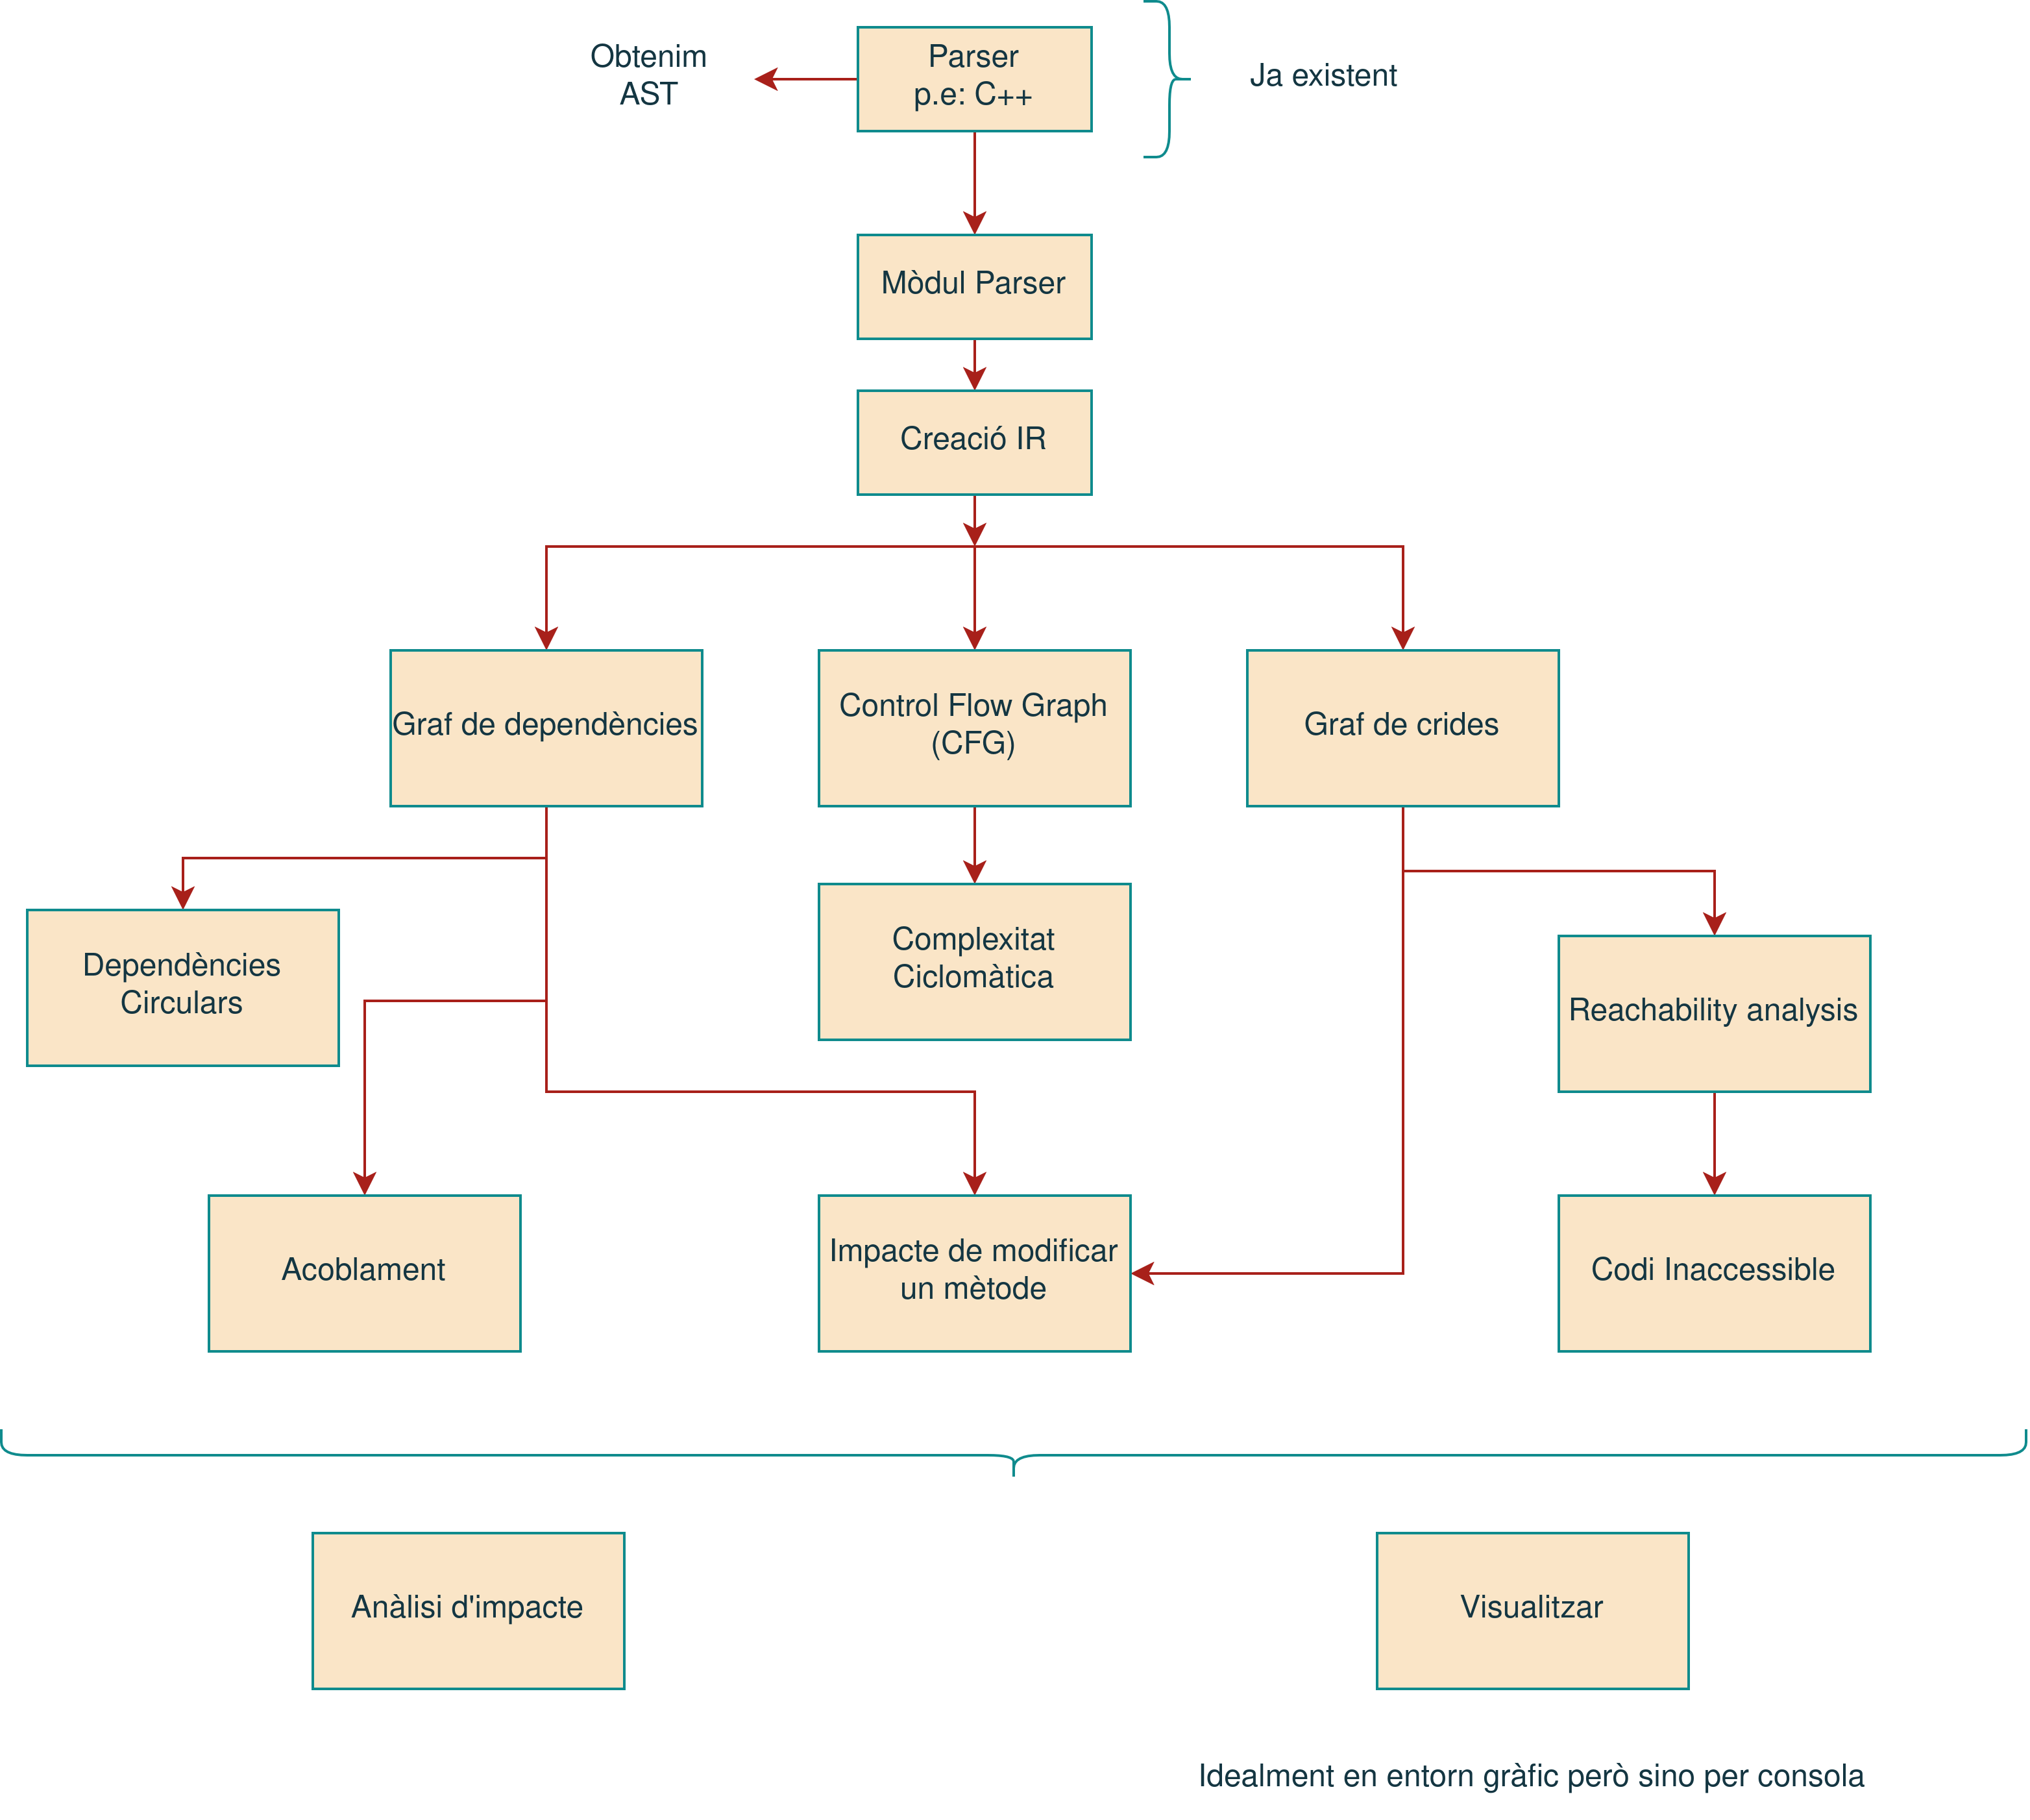
\includegraphics[width=0.8\textwidth]{figures/estructura_general_TFG.png}
    \caption{Esquema de l'arquitectura general de l'eina.}
    \label{fig:arquitectura}
\end{figure}